% !TEX root = ../../../Masterthesis.tex
\section{Red Alert}
%-----------------------------------------------------------------------------
% A
%-----------------------------------------------------------------------------
\begin{figure*}[h!]
\center
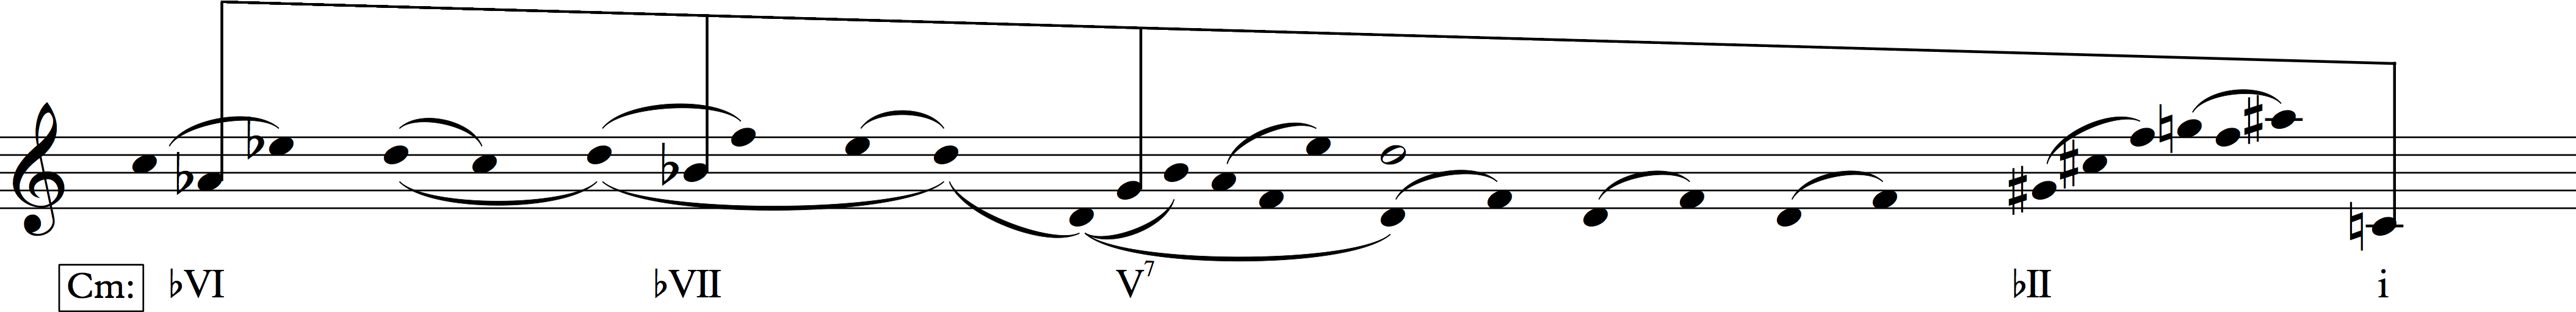
\includegraphics[width=\linewidth]{ST8_schenker_A}
	\caption{ST 8: Red Alert A: Prolonged Aeolian Cadence.}
	\label{ST8_schenker_A}
	%\setfloatalignment{b}
\end{figure*}

\noindent Picard and the crew onboard the Enterprise have just witnessed, by way of audio, the beginning of the Borg attack on earth. Picard is helpless, being several lightyears away. Determined to do something, Picard orders his crew to prepare to enter warp speed toward earth. The main theme of the film plays while Picard orders ``all hands" to battle stations. As soon as we see the Enterprise, the Star Trek theme is played, making a quick \ac{MTTP} to \ciss before landing on m.8: Cm.

%-----------------------------------------------------------------------------
% Klingon
%-----------------------------------------------------------------------------
\begin{figure}[h!]
\center
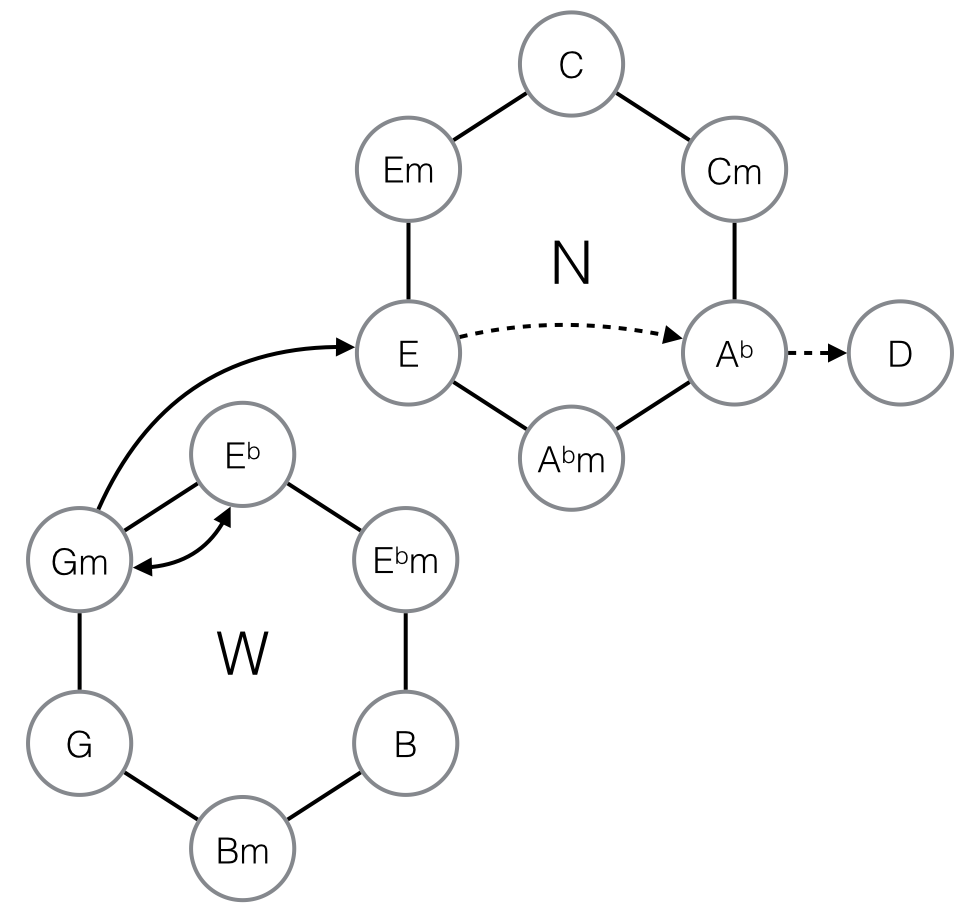
\includegraphics[width=0.7\linewidth]{ST8_red_alert_D}
	\caption{ST 8: Red Alert Klingon}
	\label{ST8_red_alert_D}
	\setfloatalignment{b}
\end{figure}

The Borg theme plays while a single Borg ship is seen fighting a number of ships from Starfleet. The battle is not unfolding in Starfleet's favor. We enter the bridge of a badly damaged ship, the USS Defiant. The crew are either dead or heavily injured. All of the sudden, the Klingon theme\footnote{written by Jerry Goldsmith for \ac{ST:TMP}.} is heard and we see Worf as he exclaims: ``Perhaps today \textit{is} a good day to die! Prepare for ramming speed!'' At that very moment, the Enterprise arrives at the battleground and intervenes, shielding the Defiant from the Borg. The music keeps Mickey-mousing, as it were, with the Star Trek theme, which is now playing to signify the presence of USS Enterprise. The theme is played twice and makes a \acf{MTTP} from \aflat to D (figure \ref{ST8_red_alert_D}).

The scene cuts to the bridge of the Enterprise and the music plays a variant of the Borg theme, m.30. The military snare drum accompanies this part, building more tension as Picard prepares and organizes the rest of the fleet for a joint strike at the Borg ship.
%-----------------------------------------------------------------------------
% Ending
%-----------------------------------------------------------------------------
As the tension in the scene builds, the music retains the tension by applying a D pedal bass throughout a series of major chords which have their foundation in the octatonic scale. This builds till part \textbf{H}, where the modified Borg theme plays, heard in m.33-39, figure \ref{ST8_red_alert_G}.

\begin{figure}
\center
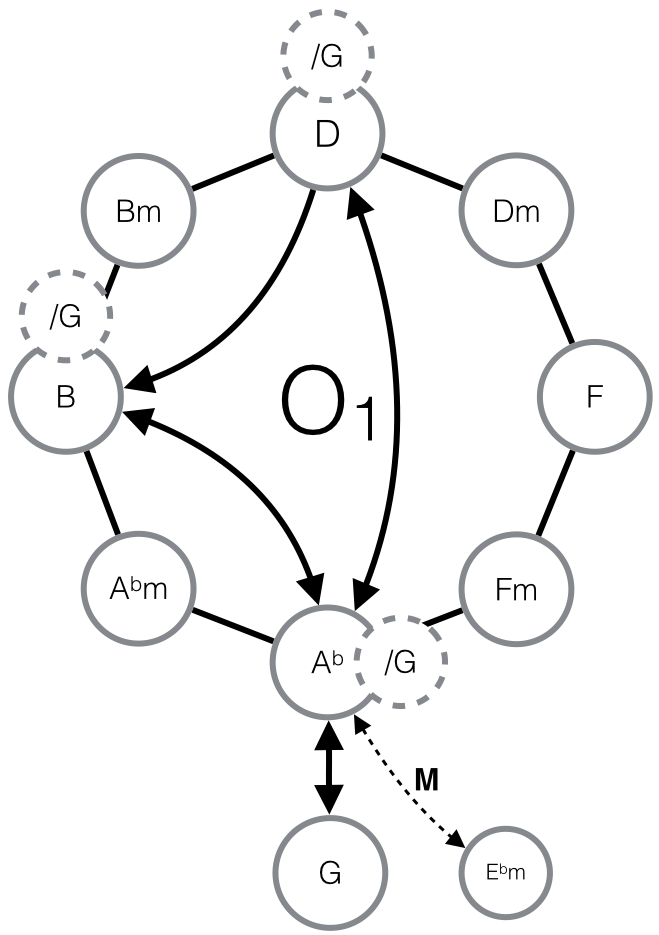
\includegraphics[width=0.5\linewidth]{ST8_red_alert_G}
	\caption{ST 8: Red Alert Ending}
	\label{ST8_red_alert_G}
	%\setfloatalignment{b}
\end{figure}


%-----------------------------------------------------------------------------
% PDF
%-----------------------------------------------------------------------------
\clearpage
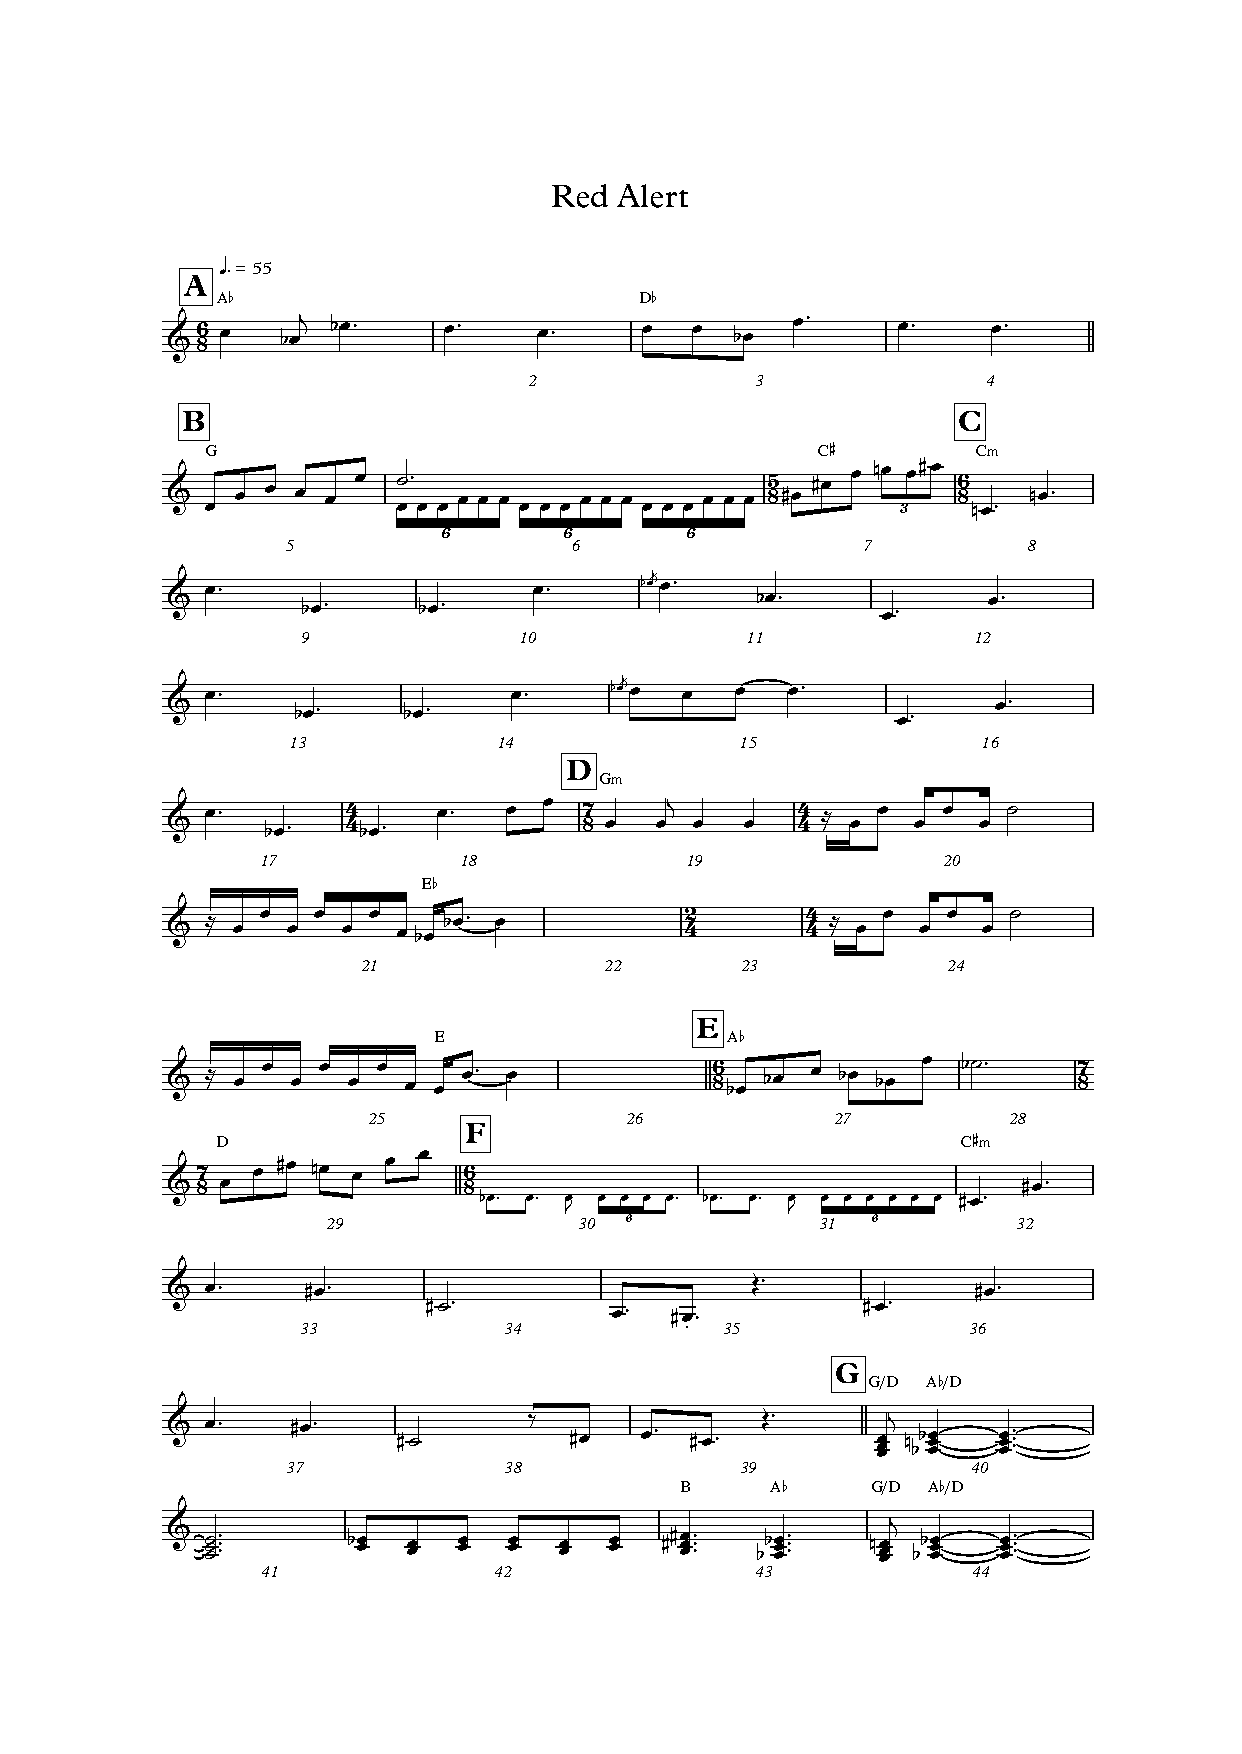
\includepdf[pages=-,pagecommand=\thispagestyle{fancy}]{pdf/st8/ST8_Red_Alert.pdf}

% Reviewed